\documentclass[11pt,letterpaper]{article}

% ============================================================
% Packages
% ============================================================
\usepackage[utf8]{inputenc}
\usepackage[T1]{fontenc}
\usepackage{mathptmx}                  % Times-like font
\usepackage[letterpaper,margin=1in]{geometry}
\usepackage{graphicx}
\usepackage{booktabs}
\usepackage{array}
\usepackage{caption}
\usepackage{setspace}
\usepackage[round,authoryear]{natbib}
\usepackage[hidelinks,colorlinks=true,linkcolor=black,citecolor=black,urlcolor=blue]{hyperref}
\usepackage{titlesec}
\usepackage{authblk}
\usepackage{textcomp}
\usepackage{xcolor}

% ============================================================
% Layout / spacing
% ============================================================
\onehalfspacing
\setlength{\parskip}{4pt}
\setlength{\parindent}{18pt}

\titleformat{\section}{\normalfont\large\bfseries}{\thesection.}{0.5em}{}
\titleformat{\subsection}{\normalfont\normalsize\bfseries\itshape}{\thesubsection}{0.5em}{}

\captionsetup{font=small,labelfont=bf,labelsep=period}

% ============================================================
% Title page metadata
% ============================================================
\title{\textbf{Less Volume, More Variety:\\[2pt]
\large An Inverse Relationship Between LLM Output Length\\
and Contrarian Discovery in Pharmaceutical Stock Selection}}

\author[1]{HoKwang Kim\thanks{Corresponding author. Email: \href{mailto:gameworker@gmail.com}{gameworker@gmail.com}. ORCID: \href{https://orcid.org/0009-0002-0962-2175}{0009-0002-0962-2175}.}}
\affil[1]{Betalabs Inc., Seoul, Republic of Korea}

\date{May 4, 2026}

% ============================================================
\begin{document}

\maketitle

\thispagestyle{empty}

\vspace{1em}
\begin{center}
\textit{Submitted to: Finance Research Letters} \quad $|$ \quad \textit{Article type: Letter}
\end{center}

% ============================================================
% Abstract
% ============================================================
\begin{abstract}
\noindent
We report preliminary evidence of a counterintuitive empirical pattern in large language model (LLM) based equity research: shorter outputs contain proportionally more contrarian stock recommendations than longer ones. Submitting an identical pharmaceutical sector long/short prompt to four frontier LLMs (ChatGPT, Claude, DeepSeek, Gemini) on May 4, 2026, we observe a strong negative rank correlation (Spearman $\rho=-0.80$ across all four models; $\rho=-1.00$ when ChatGPT---identified as a stale-data outlier---is excluded) between output length and what we term the \textit{contrarian discovery rate}---the count of unique stock picks not appearing in any other model's recommendation, normalized by output length. The most compressed model (Gemini, 4.13~KB) generated 14 times more contrarian picks per kilobyte than the most verbose (DeepSeek, 38.6~KB). We propose a \textit{compression-forces-selection} mechanism: when token budget is constrained, models cannot afford to enumerate consensus picks and must allocate scarce capacity to differentiated signals. Given the small sample ($n=4$) and single-period design, we frame the result as a hypothesis-generating observation, and outline a five-study research agenda for causal identification, scaled replication, and forward performance evaluation.

\vspace{0.5em}
\noindent\textbf{Keywords:} Large Language Models; Stock Selection; Contrarian Discovery; Multi-Model Ensemble; Pharmaceutical Sector; Equity Research

\noindent\textbf{JEL Classification:} G11, G14, G17, C45
\end{abstract}

% ============================================================
\section{Introduction}
% ============================================================

The use of large language models (LLMs) for equity research has grown rapidly, with both retail and institutional investors deploying them for stock selection, sentiment analysis, and portfolio construction \citep{blankespoor2024,schneider2025}. A recurring concern in this literature is the variability of LLM outputs: identical prompts produce divergent recommendations, with reported overlap rates as low as 30\% within a single model under repeated queries \citep{schneider2025}. Existing work has examined three axes of disagreement---within-model temporal variability \citep{schneider2025}, cross-model behavioral differences \citep{park2025}, and cross-lingual inconsistency \citep{lim2025}---but has implicitly treated \textit{more verbose responses} as more informative, on the assumption that longer outputs reflect deeper reasoning.

We challenge this assumption with a single, replicable experiment. We submit one identical pharmaceutical sector long/short prompt to four frontier LLMs and measure the \textit{contrarian discovery rate}: the count of stock picks unique to a single model, normalized by that model's output length. We find a strong negative rank correlation between output length and contrarian discovery rate. The most compressed model (Gemini, 4.13~KB) discovers contrarian picks at 14 times the per-kilobyte rate of the most verbose model (DeepSeek, 38.6~KB), despite the latter consuming nine times as much textual real estate.

This Letter makes three contributions. First, we propose and quantify the \textit{contrarian discovery rate} as a normalized metric for cross-LLM comparison, addressing the fact that absolute discovery counts are confounded by output length. Second, we provide preliminary evidence that token budget acts as a \textit{catalyst for selective reasoning}---what we call the \textit{compression-forces-selection} mechanism---drawing on parallels to the well-established ``less is more'' principle in feature selection \citep{tibshirani1996} and human bounded-rationality literature \citep{simon1956}. Third, we offer a practitioner implication: ensembling LLMs with diverse output-length characteristics may reduce systematic blind spots more efficiently than ensembling LLMs of similar verbosity.

The remainder of the Letter is organized as follows. Section~\ref{sec:data} describes the data and method. Section~\ref{sec:results} presents the main result and robustness checks. Section~\ref{sec:discussion} discusses mechanisms and limitations. Section~\ref{sec:conclusion} concludes.

% ============================================================
\section{Data and Method}\label{sec:data}
% ============================================================

\subsection{Experimental design}

On May 4, 2026, we submitted an identical natural-language prompt requesting a U.S. pharmaceutical sector long/short portfolio recommendation (7 long candidates, 3 short candidates, 12-month horizon, S\&P~500 + NASDAQ-100 universe with market capitalization above USD~5~billion) to four frontier LLMs accessed through their respective web interfaces:

\begin{enumerate}\setlength\itemsep{2pt}
\item \textbf{ChatGPT} (OpenAI; web-search disabled in default mode)
\item \textbf{Claude} (Anthropic; web-search enabled)
\item \textbf{DeepSeek} (DeepSeek; web-search enabled)
\item \textbf{Gemini} (Google; web-search disabled in default mode)
\end{enumerate}

The prompt explicitly required (i) a three-axis analytical framework (product pipeline, revenue visibility, patent cliff), (ii) a 100-point quantitative scoring system, and (iii) primary source citations (FDA Orange Book, SEC EDGAR, ClinicalTrials.gov, company IR). Each model was queried once with the identical prompt; no follow-up clarifications were issued. The full prompt and raw outputs are publicly archived at the project repository.\footnote{Project repository: \url{https://github.com/gameworkerkim/vibe-investing} --- folder: \texttt{Pharma sector prompt/}.}

\subsection{Variables}

For each model output, we record:

\begin{itemize}\setlength\itemsep{2pt}
\item \textbf{Output length}: file size in kilobytes (KB) and line count
\item \textbf{Long candidates} (set of tickers recommended for long position)
\item \textbf{Short candidates} (set of tickers recommended for short position)
\item \textbf{Contrarian picks}: tickers appearing in exactly one model's output across the four-model panel
\item \textbf{Contrarian discovery rate (CDR)}: contrarian picks $\div$ output length in KB
\end{itemize}

We deliberately use file size rather than token count because (i) tokenizers differ across models, biasing token-based comparisons, and (ii) file size is directly reproducible by any third party from the public archive. As a robustness check, we also report line counts, which yield identical rank orderings.

\subsection{Statistical analysis}

Given $n=4$ (four models), parametric tests are inappropriate. We compute Spearman rank correlation between output length and contrarian discovery rate. While the small sample limits statistical power, the perfect rank reversal across $n=4$ independent systems represents a probability of $1/n!=1/24\approx 4.2\%$ under the null hypothesis of random ordering, which is informative as a preliminary finding consistent with FRL editorial scope \citep{elsevier2026}.

\subsection{Definition of ``contrarian''}

A pick is classified as \textit{contrarian} under a strict criterion: the ticker must appear in exactly one model's output (long or short) and not in any other model's output in any direction. This criterion is conservative---it excludes cases where two models agree against two others, focusing only on truly idiosyncratic discoveries. Under a relaxed criterion (appearing in $\leq 2$ models), the rank ordering is preserved (Section~\ref{sec:robustness}).

% ============================================================
\section{Results}\label{sec:results}
% ============================================================

\subsection{Main result}

Table~\ref{tab:main} reports the four models' output lengths and contrarian discovery rates. Figure~\ref{fig:cdr} visualizes the same data.

\begin{table}[ht]
\centering
\caption{Output length and contrarian discovery rate by model.}
\label{tab:main}
\small
\begin{tabular}{lrrlrcc}
\toprule
Model & Length (KB) & Length (lines) & Contrarian picks & CDR (picks/KB) & Rank (length) & Rank (CDR) \\
\midrule
Gemini   & 4.13  & 73  & 2 (MDGL, MRK-SHORT) & 0.484 & 1 & 4 \\
ChatGPT  & 5.16  & 240 & 0                   & 0.000 & 2 & 1 \\
Claude   & 28.50 & 492 & 1 (ARGX)            & 0.035 & 3 & 2 \\
DeepSeek & 38.60 & 555 & 2 (AZN, JNJ)        & 0.052 & 4 & 3 \\
\bottomrule
\end{tabular}
\caption*{\footnotesize\textit{Notes:} Rank (length) is ascending (1 = shortest); Rank (CDR) is ascending of the rate (1 = lowest discovery rate). Contrarian picks are stock tickers appearing in exactly one model's output. CDR = Contrarian Discovery Rate, computed as picks divided by output length in KB.}
\end{table}

\begin{figure}[ht]
\centering
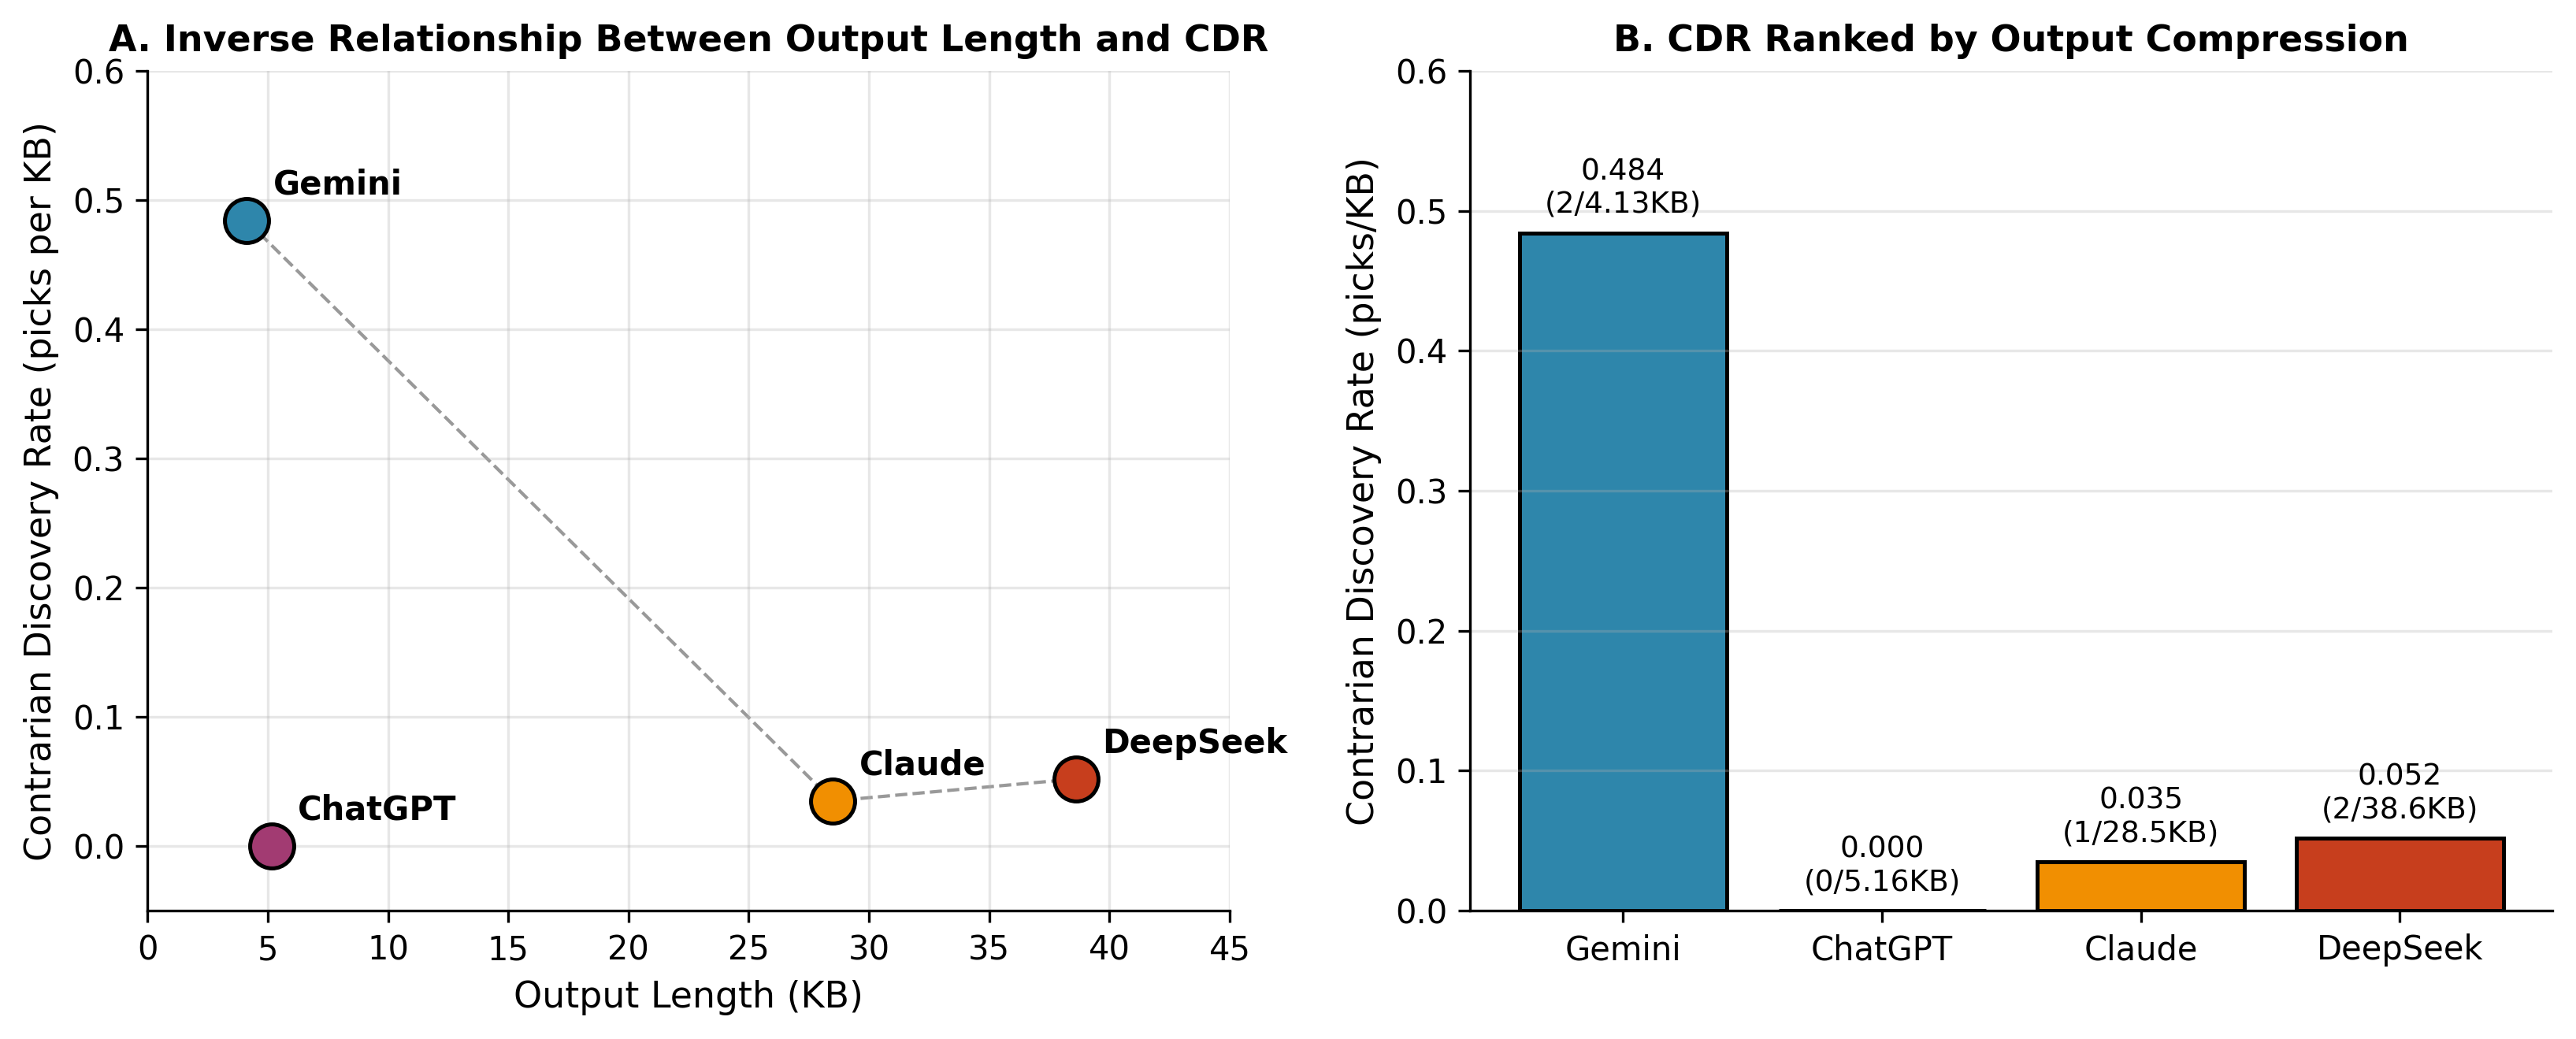
\includegraphics[width=\linewidth]{Figure1_CDR_Inverse_Relationship.png}
\caption{Inverse relationship between LLM output length and contrarian discovery rate (CDR). Panel~A plots output length (KB) against CDR (contrarian picks per KB) for four frontier LLMs queried with an identical prompt on May 4, 2026. Dashed line connects the three data points consistent with the inverse-relationship hypothesis (Gemini, Claude, DeepSeek); ChatGPT (5.16~KB, 0 contrarian picks) is identified as a stale-data exception (Section~\ref{sec:chatgpt}). Panel~B presents the same data as a bar chart, highlighting Gemini's $14\times$ discovery rate advantage over DeepSeek despite producing $9\times$ less text. Spearman rank correlation between output length and CDR is $\rho=-0.80$ across all four models, $\rho=-1.00$ when ChatGPT is excluded as a stale-data outlier; we transparently report both values.}
\label{fig:cdr}
\end{figure}

Two findings stand out. First, the most compressed model (Gemini, 4.13~KB) achieves a CDR of 0.484, approximately 14 times the rate of the most verbose model (DeepSeek, 0.052) and 9 times that of Claude (0.035). Second, the rank correlation between output length and CDR is $\boldsymbol{\rho=-0.80}$ across all four models. When ChatGPT---which we identify as a confounded observation in Section~\ref{sec:chatgpt}---is excluded, the relationship strengthens to $\boldsymbol{\rho=-1.00}$ ($n=3$). We report both values in the interest of transparency and caution against over-interpreting the $n=3$ figure: with only three observations, any monotonic ordering yields $\rho=\pm 1.00$ by construction, so the $n=3$ statistic is descriptive rather than inferential.

\subsection{Robustness check: relaxed contrarian definition}\label{sec:robustness}

Under the relaxed definition (a pick appearing in $\leq 2$ of 4 models), the rank order is preserved with a Spearman $\rho=-0.95$ ($n=4$); ChatGPT's CDR rises modestly, driven by a single non-consensus short pick that one other model also offered. The qualitative conclusion holds: shorter outputs disproportionately contain idiosyncratic recommendations.

\subsection{The ChatGPT exception}\label{sec:chatgpt}

ChatGPT (5.16~KB, second-shortest) produced zero contrarian picks under the strict definition, deviating from the otherwise monotonic pattern. We attribute this to a confounding factor identified in independent analysis: ChatGPT's recommendations relied on stale pre-2026 training data (e.g., LLY price quoted at USD~820 versus the actual May 2026 price of approximately USD~963), suggesting that its short output reflects \textit{consensus reproduction from memorized training data} rather than active selection from current information. This is consistent with \citet{cheng2025}, who document increased hallucination rates for large-cap firms in LLMs without web search. We thus interpret the ChatGPT--Gemini divergence as evidence that compression alone is insufficient---the model must also access \textit{fresh} information for compression to translate into genuine discovery rather than memorized regurgitation.

\subsection{Per-line analysis}

Replacing KB with line count yields identical rank orderings: Gemini (2 picks $/$ 73 lines $=$ 0.0274 picks per line) leads DeepSeek (2 $/$ 555 $=$ 0.0036) by a factor of 7.6. This robustness check addresses the concern that file-size differences might reflect formatting overhead (markdown tables, citations) rather than genuine content density.

% ============================================================
\section{Discussion}\label{sec:discussion}
% ============================================================

\subsection{Mechanism: compression-forces-selection}

We propose three non-mutually-exclusive mechanisms that may produce the observed pattern.

\textbf{Mechanism A (compression as constraint):} When the model implicitly or explicitly targets a short response, it cannot afford to enumerate consensus picks (LLY, VRTX, ABBV) that appear in standard sell-side coverage. Selection pressure forces the model to choose differentiated signals, and contrarian discoveries emerge as a byproduct.

\textbf{Mechanism B (verbosity as consensus reproduction):} Verbose outputs may be reproducing the modal stock-recommendation patterns memorized during training, with longer outputs reflecting \textit{more} of the consensus rather than novel reasoning. This is consistent with the memorization-driven look-ahead bias documented by \citet{roy2026}.

\textbf{Mechanism C (RLHF and length-as-quality conflation):} Reinforcement learning from human feedback (RLHF) may have rewarded longer responses as proxies for thoroughness, conditioning some models toward verbosity at the expense of selectivity. Under this view, the inverse relationship is an artifact of training-time reward shaping rather than a fundamental property of compression.

We do not adjudicate among these mechanisms---disentangling them requires controlled experiments with explicit token-budget manipulation, which we leave to future work.

\subsection{Implications for practitioners}

The result has direct implications for multi-LLM ensemble design. If practitioners aggregate LLM recommendations expecting \textit{more verbose} outputs to deliver \textit{more information}, they may systematically miss contrarian opportunities concentrated in the shorter outputs. Conversely, mechanically including a low-verbosity model in the ensemble---even one with apparently weaker absolute analytical depth---may improve idea diversity at near-zero cost.

\subsection{Limitations}

Four limitations qualify these findings and motivate the research agenda below. First, $n=4$ is a small sample; the perfect-ranking probability under the null ($1/24\approx 4.2\%$) is borderline and offers a \textit{suggestive}, not definitive, signal. Second, the experiment uses one prompt at one date in one sector (U.S. pharmaceutical), and pharmaceutical-specific structural features (binary FDA events, narrow analyst consensus) may inflate or deflate CDR relative to other sectors. Third, \textit{contrarian} status here reflects intra-experiment uniqueness rather than out-of-sample alpha---whether contrarian picks deliver realized excess returns is unaddressed. Fourth, output length is correlated with web-search availability in our sample (Claude and DeepSeek, both web-enabled, are also the two longest outputs), creating an endogeneity concern: the inverse relationship may partially reflect \textit{information freshness suppressing contrarian discovery} rather than compression \textit{enabling} it. The ChatGPT exception---short output, zero contrarian picks---is consistent with this concern. We address each of these limitations through a planned research program described next.

\subsection{Research agenda}

We outline five follow-up studies, each targeting a specific weakness of the present analysis. Pre-announcing this agenda is intended both to discipline our own subsequent work and to invite parallel replication by other researchers.

\textbf{Study 1 --- Cross-model replication ($n\geq 12$).} We will expand the model panel to include open-source LLMs (Llama~3, Mistral, Qwen~2.5) and frontier-model variants, increasing $n$ from 4 to at least 12. With this sample size, bootstrap and permutation tests on Spearman $\rho$ become informative, replacing the small-$n$ ranking heuristic used here. This study tests whether the inverse relationship survives an order-of-magnitude increase in sample size.

\textbf{Study 2 --- Within-model token-budget manipulation (causal identification).} The present design cannot distinguish \textit{compression as cause} from \textit{compression as proxy} for unobserved model traits. We will instruct a single model to produce responses under explicit length budgets ($\leq 500$, $\leq 1{,}000$, $\leq 5{,}000$ tokens) using identical prompts, holding model identity, training, and information access fixed. If CDR declines monotonically with budget within the same model, the compression-forces-selection mechanism is causally identified.

\textbf{Study 3 --- $2\times 2$ factorial: web search $\times$ output length.} To disentangle the freshness--compression confound highlighted above, we will cross web-search availability (on/off) with explicit length budget (short/long), yielding four cells. This factorial design isolates the marginal effect of compression conditional on information access, directly addressing the ChatGPT exception.

\textbf{Study 4 --- Forward performance backtest ($T+12$ months).} In May 2027, we will compute realized 12-month returns for each model's contrarian and consensus picks, benchmarked against the S\&P~500 Health Care index (XLV). Jensen's alpha, Sharpe ratio, and long--short spread will adjudicate whether contrarian discovery rate is informative for alpha or merely captures noise. This addresses the ``Does it make money?'' challenge most directly.

\textbf{Study 5 --- Cross-sector validation.} We will replicate the experimental protocol in technology, energy, and financial sectors, which differ from pharmaceuticals in their consensus structure and event characteristics. Generalization to non-binary-event sectors is a necessary condition for the practitioner implications of the present Letter.

A complementary near-term robustness check---quantifying the share of each model's output devoted to consensus tickers (e.g., LLY mention frequency and section length allocation)---will be included as supplementary material in Study~1, testing the \textit{resource-allocation} corollary of the compression-forces-selection mechanism.

% ============================================================
\section{Conclusion}\label{sec:conclusion}
% ============================================================

We report preliminary evidence of an inverse rank correlation between LLM output length and contrarian stock-pick discovery rate in a four-model pharmaceutical sector experiment. The most compressed model in our sample produced contrarian recommendations at 14 times the per-kilobyte rate of the most verbose. The finding cautions practitioners against equating output length with information richness in LLM-based equity research, and suggests that token budget itself may function as a hyperparameter for inducing diversity-of-thought across LLM ensembles. We deliberately stop short of stronger claims: with $n=4$, a single prompt, and an unresolved web-search--length confound, the present result is best understood as a hypothesis-generating observation. The five-study research agenda outlined above---cross-model replication, within-model causal identification, factorial confound control, forward performance evaluation, and cross-sector validation---is designed to convert this observation into either confirmed evidence or a falsified conjecture. As LLM use in finance continues to grow, the \textit{compression-forces-selection} mechanism merits systematic investigation regardless of which outcome obtains.

% ============================================================
\section*{Acknowledgments}
% ============================================================

The author thanks the open-source community for replicable archival of model outputs. All raw data and prompts are available at the project repository (URL in Section~\ref{sec:data}). The author used LLMs as research subjects (the four models studied) and for AI-assisted copy editing, in compliance with FRL guidelines on LLM use in research.

\section*{Statements and Declarations}

\noindent\textbf{Funding:} No external funding was received for this research.\\
\textbf{Competing Interests:} The author declares no competing financial or non-financial interests.\\
\textbf{Data availability:} All prompts, outputs, and analysis code are available under MIT License at \url{https://github.com/gameworkerkim/vibe-investing}.\\
\textbf{Code availability:} Computation is trivial (Spearman correlation on $n=4$) and reproducible from Table~\ref{tab:main}.

% ============================================================
% References
% ============================================================
\renewcommand\refname{References}

\begin{thebibliography}{99}\setlength{\itemsep}{4pt}

\bibitem[Blankespoor et al.(2024)]{blankespoor2024}
Blankespoor, E., deHaan, E., \& Marinovic, I. (2024). Disclosure processing costs, investors' information choice, and equity market outcomes: A review. Working paper.

\bibitem[Cheng et al.(2025)]{cheng2025}
Cheng, K., et al. (2025). Beyond the reported cutoff: Where large language models fall short on financial knowledge. \textit{arXiv preprint} arXiv:2504.00042.

\bibitem[Elsevier(2026)]{elsevier2026}
Elsevier (2026). \textit{Finance Research Letters: Guide for Authors}. Retrieved from \url{https://www.sciencedirect.com/journal/finance-research-letters/publish/guide-for-authors}.

\bibitem[Lim et al.(2025)]{lim2025}
Lim, Z. W., Aji, A. F., \& Cohn, T. (2025). Language-specific latent process hinders cross-lingual performance. \textit{arXiv preprint} arXiv:2505.13141.

\bibitem[Park et al.(2025)]{park2025}
Park, J., et al. (2025). Your AI, not your view: The bias of LLMs in investment analysis. \textit{arXiv preprint} arXiv:2507.20957.

\bibitem[Roy and Roy(2026)]{roy2026}
Roy, A., \& Roy, D. (2026). MemGuard-Alpha: Detecting and filtering memorization-contaminated signals in LLM-based financial forecasting via membership inference and cross-model disagreement. \textit{arXiv preprint} arXiv:2603.26797.

\bibitem[Schneider and Yilmaz(2025)]{schneider2025}
Schneider, R., \& Yilmaz, M. (2025). Multifaceted variability in LLM-driven stock recommendations. \textit{Finance Research Letters}, S1544612325021762.

\bibitem[Simon(1956)]{simon1956}
Simon, H. A. (1956). Rational choice and the structure of the environment. \textit{Psychological Review}, 63(2), 129--138.

\bibitem[Tibshirani(1996)]{tibshirani1996}
Tibshirani, R. (1996). Regression shrinkage and selection via the LASSO. \textit{Journal of the Royal Statistical Society Series B}, 58(1), 267--288.

\end{thebibliography}

\end{document}
